\documentclass[border=5pt]{standalone}
\usepackage{tikz}
\usepackage{xcolor}

\definecolor{danger}{RGB}{220,53,69}
\definecolor{warning}{RGB}{255,193,7}
\definecolor{secondary}{RGB}{108,117,125}
\definecolor{success}{RGB}{40,167,69}

\begin{document}
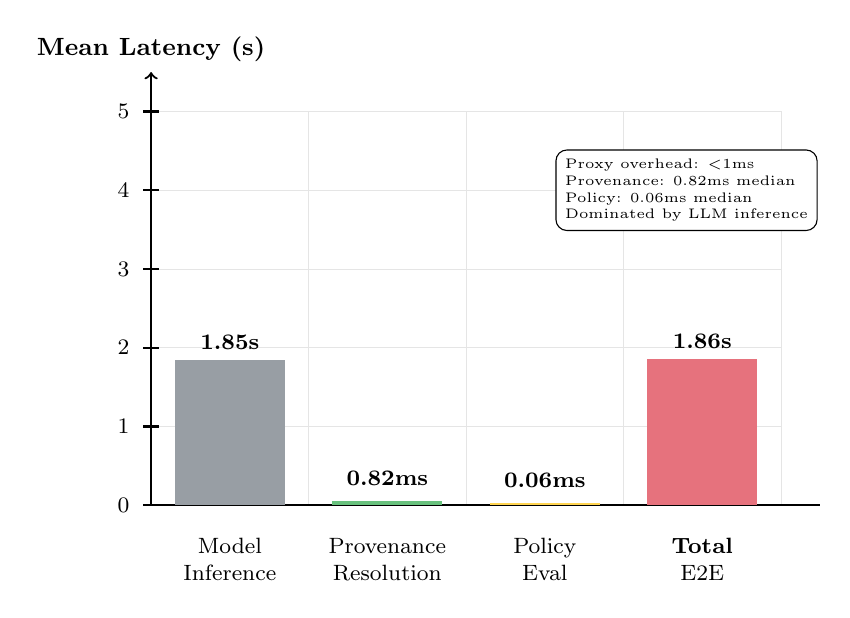
\begin{tikzpicture}[scale=1]
  % Background grid
  \draw[gray!20, very thin] (0,0) grid[xstep=2, ystep=1] (8,5);
  
  % Y-axis (Latency in seconds)
  \draw[thick, ->] (0,0) -- (0,5.5) node[above, font=\small\bfseries] {Mean Latency (s)};
  \foreach \y/\label in {0/0, 1/1, 2/2, 3/3, 4/4, 5/5} {
    \draw[thick] (-0.1,\y) -- (0.1,\y);
    \node[left, font=\footnotesize] at (-0.15,\y) {\label};
  }
  
  % X-axis
  \draw[thick] (0,0) -- (8.5,0);
  
  % Bar positions and widths
  \def\barwidth{1.4}
  
  % Model Inference: 1.85s -> 1.85
  \fill[secondary!70] (1-\barwidth/2, 0) rectangle (1+\barwidth/2, 1.85);
  \node[below, font=\footnotesize, align=center] at (1, -0.3) {Model\\Inference};
  \node[above, font=\footnotesize\bfseries] at (1, 1.85) {1.85s};
  
  % Provenance Resolution: 0.82ms -> bar at ~0.001s (negligible, use min visible)
  \fill[success!70] (3-\barwidth/2, 0) rectangle (3+\barwidth/2, 0.05);
  \node[below, font=\footnotesize, align=center] at (3, -0.3) {Provenance\\Resolution};
  \node[above, font=\footnotesize\bfseries] at (3, 0.12) {0.82ms};
  
  % Policy Eval: 0.06ms -> bar negligible
  \fill[warning!70] (5-\barwidth/2, 0) rectangle (5+\barwidth/2, 0.03);
  \node[below, font=\footnotesize, align=center] at (5, -0.3) {Policy\\Eval};
  \node[above, font=\footnotesize\bfseries] at (5, 0.10) {0.06ms};
  
  % Total E2E: 1.86s (dominated by LLM)
  \fill[danger!70] (7-\barwidth/2, 0) rectangle (7+\barwidth/2, 1.86);
  \node[below, font=\footnotesize, align=center] at (7, -0.3) {\textbf{Total}\\E2E};
  \node[above, font=\footnotesize\bfseries] at (7, 1.86) {1.86s};
  
  % Breakdown annotation
  \node[draw, rounded corners, fill=white, font=\tiny, align=left] 
    at (6.8, 4) {Proxy overhead: $<$1ms\\Provenance: 0.82ms median\\Policy: 0.06ms median\\Dominated by LLM inference};
  
\end{tikzpicture}
\end{document}
